\documentclass{beamer}
\usepackage[T1]{fontenc}
\usepackage[utf8]{inputenc}
\usepackage{lmodern}
\usepackage[polish]{babel}
\usepackage{graphicx}

\usetheme{AGH}

\title[Interpolacja obrazu barwnego]{Równoległa interpolacja obrazu barwnego
  z~kamery cyfrowej}

\author[B. Bułat, T. Drzewiecki]{Bartłomiej Bułat, Tomasz Drzewiecki}

\date[2011]{24.01.2012}

\institute[AGH]
{Wydział EAIiIB\\ 
Katedra Automatyki i Inżynierii Biomedycznej
}

\setbeamertemplate{itemize item}{$\maltese$}

\begin{document}

{
\usebackgroundtemplate{
\includegraphics[width=\paperwidth]{titlepagepl}} % wersja polska
 \begin{frame}
   \titlepage
 \end{frame}
}

%---------------------------------------------------------------------------

%% Figure example
%\begin{figure}
%  \includegraphics[width=0.5\textwidth]{filename}
%  \caption{Figure caption}
%  \label{fig:label}
%\end{figure}

\begin{frame}
\frametitle{Wstęp}

\end{frame}

\begin{frame}
  \frametitle{Implementacja kontrollera po stronie CPU}
  W~celu łatwiejszej, szybszej oraz generującej mniej błędów implementacji stworzono maly framework klas realizujących obsługę OpenCL od strony procesora.
Schemat jego struktury jest przedstawiony na rys. \ref{fig:class_diagram} na następnym slajdzie.
\end{frame}

\begin{frame}
  \frametitle{Diagram klas}
\begin{figure}
  \centering
  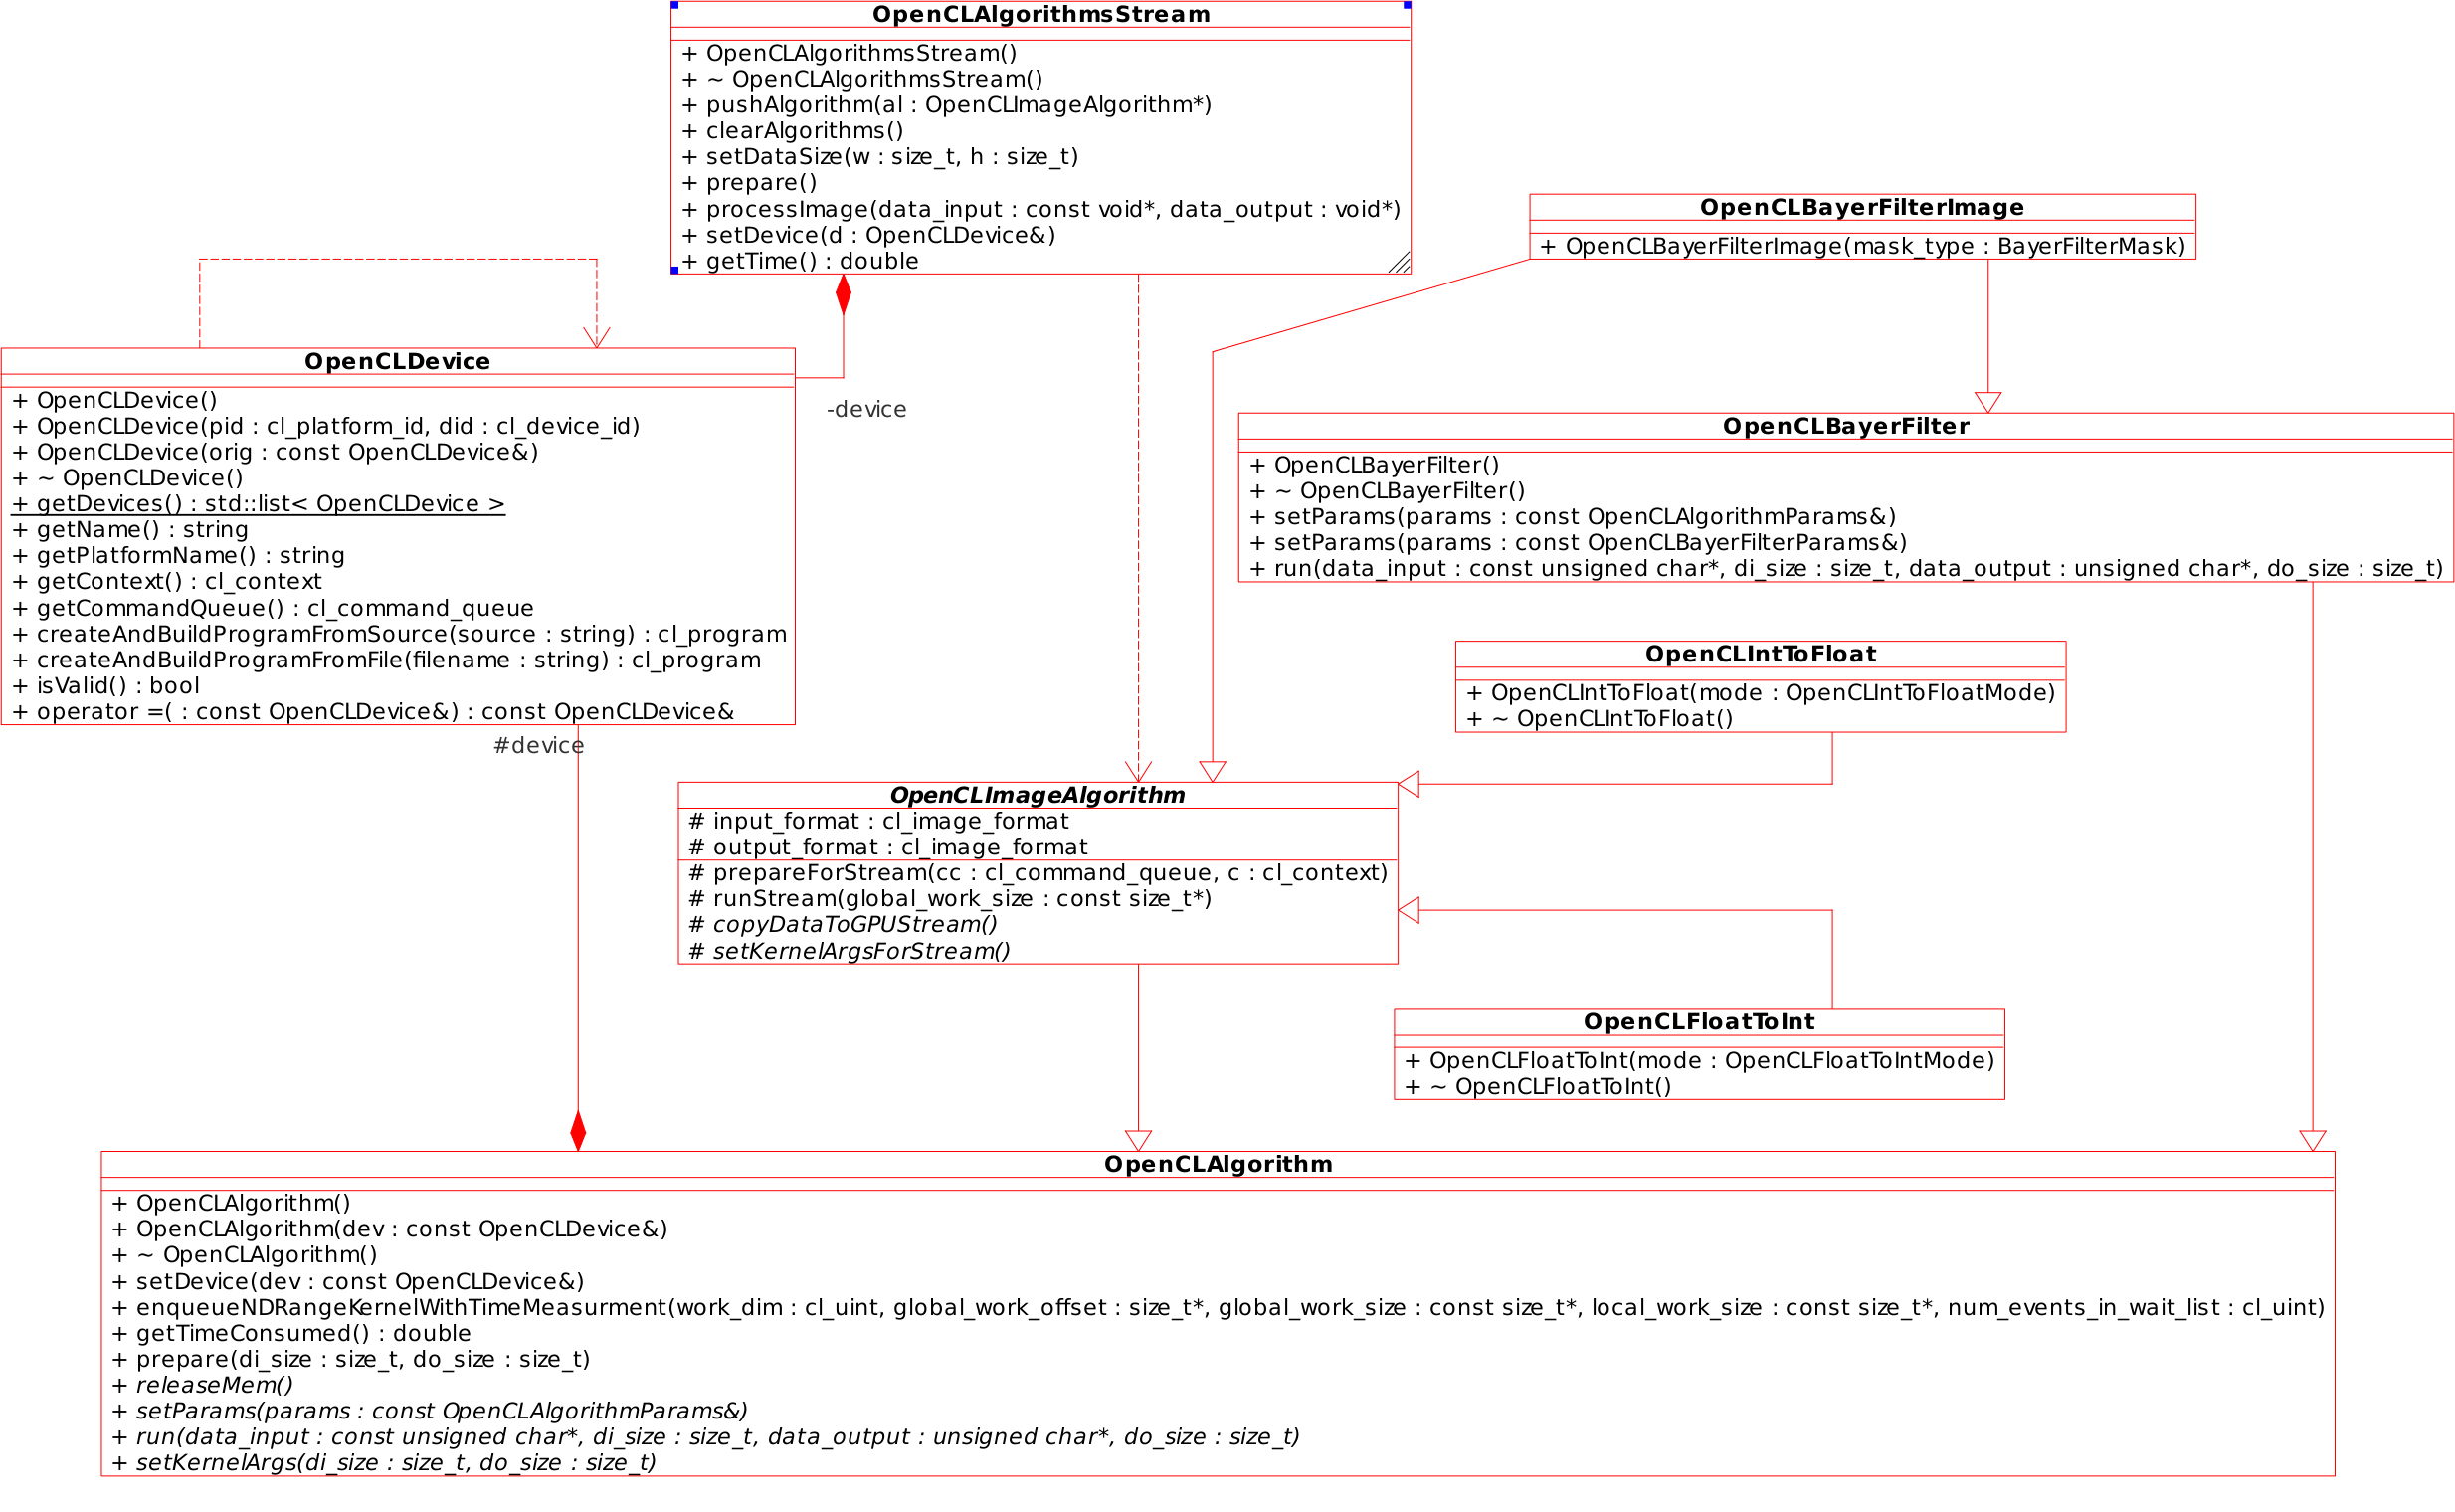
\includegraphics[width=0.6\linewidth]{class_diagram}
  \caption{Diagram klas stworzonego frameworku.}
  \label{fig:class_diagram}
\end{figure}
  
\end{frame}

\begin{frame}
  \frametitle{Testowanie}
  Testy algorytmu zostały zrealizowane z użyciem dwóch kart graficznych o~parametrach:
\begin{center}
   \begin{tabular}{ |l | l | l | }
     \hline
       & GT 555M & GT9800 \\ \hline
     Liczba rdzeni & 144 & 128 \\ \hline
     Częstotliwość rdzenia & 1250MHz & 600MHz \\ \hline
     Częstotliwość pamięci & 1800MHz & 900MHz \\ \hline
     Magistrala pamięci & 128bit & 256bit \\ \hline
   \end{tabular}
\end{center}
\end{frame}
\begin{frame}
  \frametitle{Podsumowanie}
  
\end{frame}
\begin{frame}
  \frametitle{Podsumowanie}
  
\end{frame}

\end{document}

